%%%%%%%%%%%%%%%%%%%%%%%%%%%%%%%%%%%%%%%%%%%%%%%%%%%%%%%%%%%%%%%%%%%%%%%%%%%%%%%%
%2345678901234567890123456789012345678901234567890123456789012345678901234567890
%        1         2         3         4         5         6         7         8

\documentclass[letterpaper, 10 pt, conference]{ieee/ieeeconf}  % Comment this line out if you need a4paper

%\documentclass[a4paper, 10pt, conference]{ieeeconf}      % Use this line for a4 paper

\IEEEoverridecommandlockouts                              % This command is only needed if 
                                                          % you want to use the \thanks command

\overrideIEEEmargins                                      % Needed to meet printer requirements.

% See the \addtolength command later in the file to balance the column lengths
% on the last page of the document

% The following packages can be found on http:\\www.ctan.org
%\usepackage{graphics} % for pdf, bitmapped graphics files
\usepackage{graphicx} % for jpg
%\usepackage{epsfig} % for postscript graphics files
%\usepackage{mathptmx} % assumes new font selection scheme installed
%\usepackage{times} % assumes new font selection scheme installed
%\usepackage{amsmath} % assumes amsmath package installed
%\usepackage{amssymb}  % assumes amsmath package installed

\usepackage[hidelinks]{hyperref}
\usepackage{todonotes}
\setlength{\marginparwidth}{1.5cm} % For TODOs.
%\usepackage[T1]{fontenc} % For less than signs?
\usepackage{subcaption}
\usepackage{dblfloatfix}
% For lovely checkmarks.
\usepackage{pifont}% http://ctan.org/pkg/pifont
\newcommand{\cmark}{\ding{51}}%
\newcommand{\xmark}{\ding{55}}%
% For footnotes in table.
\usepackage{threeparttable}

%%%%%%%%%%%%%%%%%%%%%%%%%%%%%%%%%%%%%%%%%%%%%%%%%%%%%%%%%%%%%%%%%%%%%%%%%%%%%%%%
\title{\LARGE \bf
A lightweight, cross-platform, multiuser robot visualization \\ using the cloud*
}

\author{William Hilton$^{1}$, Dan Lofaro$^{2}$, and Youngmoo Kim$^{3}$% <-this % stops a space
\thanks{*This work was supported in part by NSF CNS-0960061: MRI-R2 Development of a Common Platform for Unifying Humanoids Research.}% <-this % stops a space
\thanks{$^{1}$William Hilton is with Department of Electrical Engineering, Drexel University,
        Philadelphia, PA 19104, USA
        {\tt\small wmhilton@drexel.edu}}%        
\thanks{$^{2}$Dan Lofaro is with Department of Electrical Engineering, George Mason University,
        Fairfax, VA 22030, USA
        {\tt\small dlofaro@gmu.edu}}%
%\thanks{$^{2}$Paul Oh is with Faculty of Mechanical Engineering, Drexel University,
%        Philadelphia, PA 19104, USA
%        {\tt\small paul@coe.drexel.edu}}%        
\thanks{$^{3}$Youngmoo Kim is with Faculty of Electrical Engineering, Drexel University,
        Philadelphia, PA 19104, USA
        {\tt\small ykim@drexel.edu}}%
}

\begin{document}
\maketitle
\thispagestyle{empty}
\pagestyle{empty}

%%%%%%%%%%%%%%%%%%%%%%%%%%%%%%%%%%%%%%%%%%%%%%%%%%%%%%%%%%%%%%%%%%%%%%%%%%%%%%%%

% % Youngmoo kim's thoughts
% Education
% Talk more about pros/cons of Firebase as a database for robot telemetry data
% Latency, race conditions? Real-time telemetry

% Explain the database aspect for Firebase more. Stores data. Triggers updates.

% Give some more example applications
% Roboticist wants an interface that's fast and easy to use
% Team 
% Audience of thousands for space rover landing on Mars.
% Show system addresses all scenarios.

% But be very specific in how you talk about the implementation.
% Don't minimize the amount of work done to make it work well. (You didn't just download 3 components and ir worked)

\begin{abstract}
Cloud robotics emphasizes harnessing the power of the Web for robotics.
Modern mobile devices connect to the Web and are convenient user interfaces.
We decided to explore what was possible at the intersection of robotics, the Web, and mobile devices by creating a mobile web interface for a humanoid robot.
This paper describes our implementation of a monitoring interface for high degree of freedom (DOF) robots that works with both desktop and mobile devices.
Using only standard web technologies, our application provides a rich 3D interface that displays the robot's pose, orientation, and sensor data, and can update at 30Hz.
It is easy to use, because there is no software for the user to install; it runs using the device's mobile browser.
The web interface can be deployed on a private or public cloud, and is designed to scale to support hundreds or thousands of viewers by utilizing cloud services.
The system was successfully tested with two different robots and on multiple browsers and mobile devices.
\end{abstract}


%%%%%%%%%%%%%%%%%%%%%%%%%%%%%%%%%%%%%%%%%%%%%%%%%%%%%%%%%%%%%%%%%%%%%%%%%%%%%%%%
\section{INTRODUCTION}
Mobile devices (smartphones and tablets) have improved so much in a few short years that they are rapidly encroaching on niches previously held by laptops and desktops.
But traditional software used in robotics research, such as the Linux console and ROS, does not lend itself to running on mobile devices.
Their user interfaces were designed for desktop screens, rely heavily on keyboard interaction, and aren't designed for touch interaction.

While desktops and laptops will undoubtedly remain the primary devices on which robotics software and algorithms are written, there are times when mobile devices would be useful.
Particularly when working with mobile robots, it makes sense to use mobile hardware.
Laptops are cumbersome to walk around with compared to a lightweight tablet.
Mobile devices then would be good for user interfaces to the robot.

However, writing software specifically for mobile devices is burdensome, because much work must be duplicated to write native apps for desktops, Android, and iOS.
Furthermore, once written, there are additional hurdles of publishing the application to the App store of the platform(s) of choice.
Web applications, in contrast are cross-platform by default.
The same code can adjust to different screen size, so you don't need to maintain separate versions for mobile and desktop.
Because it is just a webpage, to update the software all you need to do is hit ``Refresh''.
For these reasons, we felt it would be best to write a web application rather than a native application.

As researchers, we were interested in developing an easy-to-use tool that would be useful to us as we worked with our own robots, Hubo 2+ \cite{park2007mechanical} and DRC Hubo\footnote{\url{http://www.drc-hubo.com/}}.  
Therefore we created interfaces to increase our situational awareness.
For instance, our 3D WebGL interface allows us to visualize the amount of force and torque on the robots arms and wrists.
We also created a second interface that presents detailed data about the joints and sensors in a table, where joints with errors would be highlighted red.
Since this was our first system, we decided to make it read-only so the interfaces are for monitoring the robot only, not controlling it.

Because the application runs in the cloud, there is enormous potential for distance collaboration and education.
Consider a massive open online course (MOOC) that teaches robotics and had a live demonstration.
Instead of merely streaming video to students, imagine they had access to a live feed from the robot's sensors and internal state.
Or perhaps for future Mars lander missions, instead of showing premade computer graphics illustrating where the lander was and what it is doing, NASA could have a web application with a 3D model of the rover that is driven in real time by the rovers's actual telemetry data.

\begin{figure}[thpb]
  \centering
  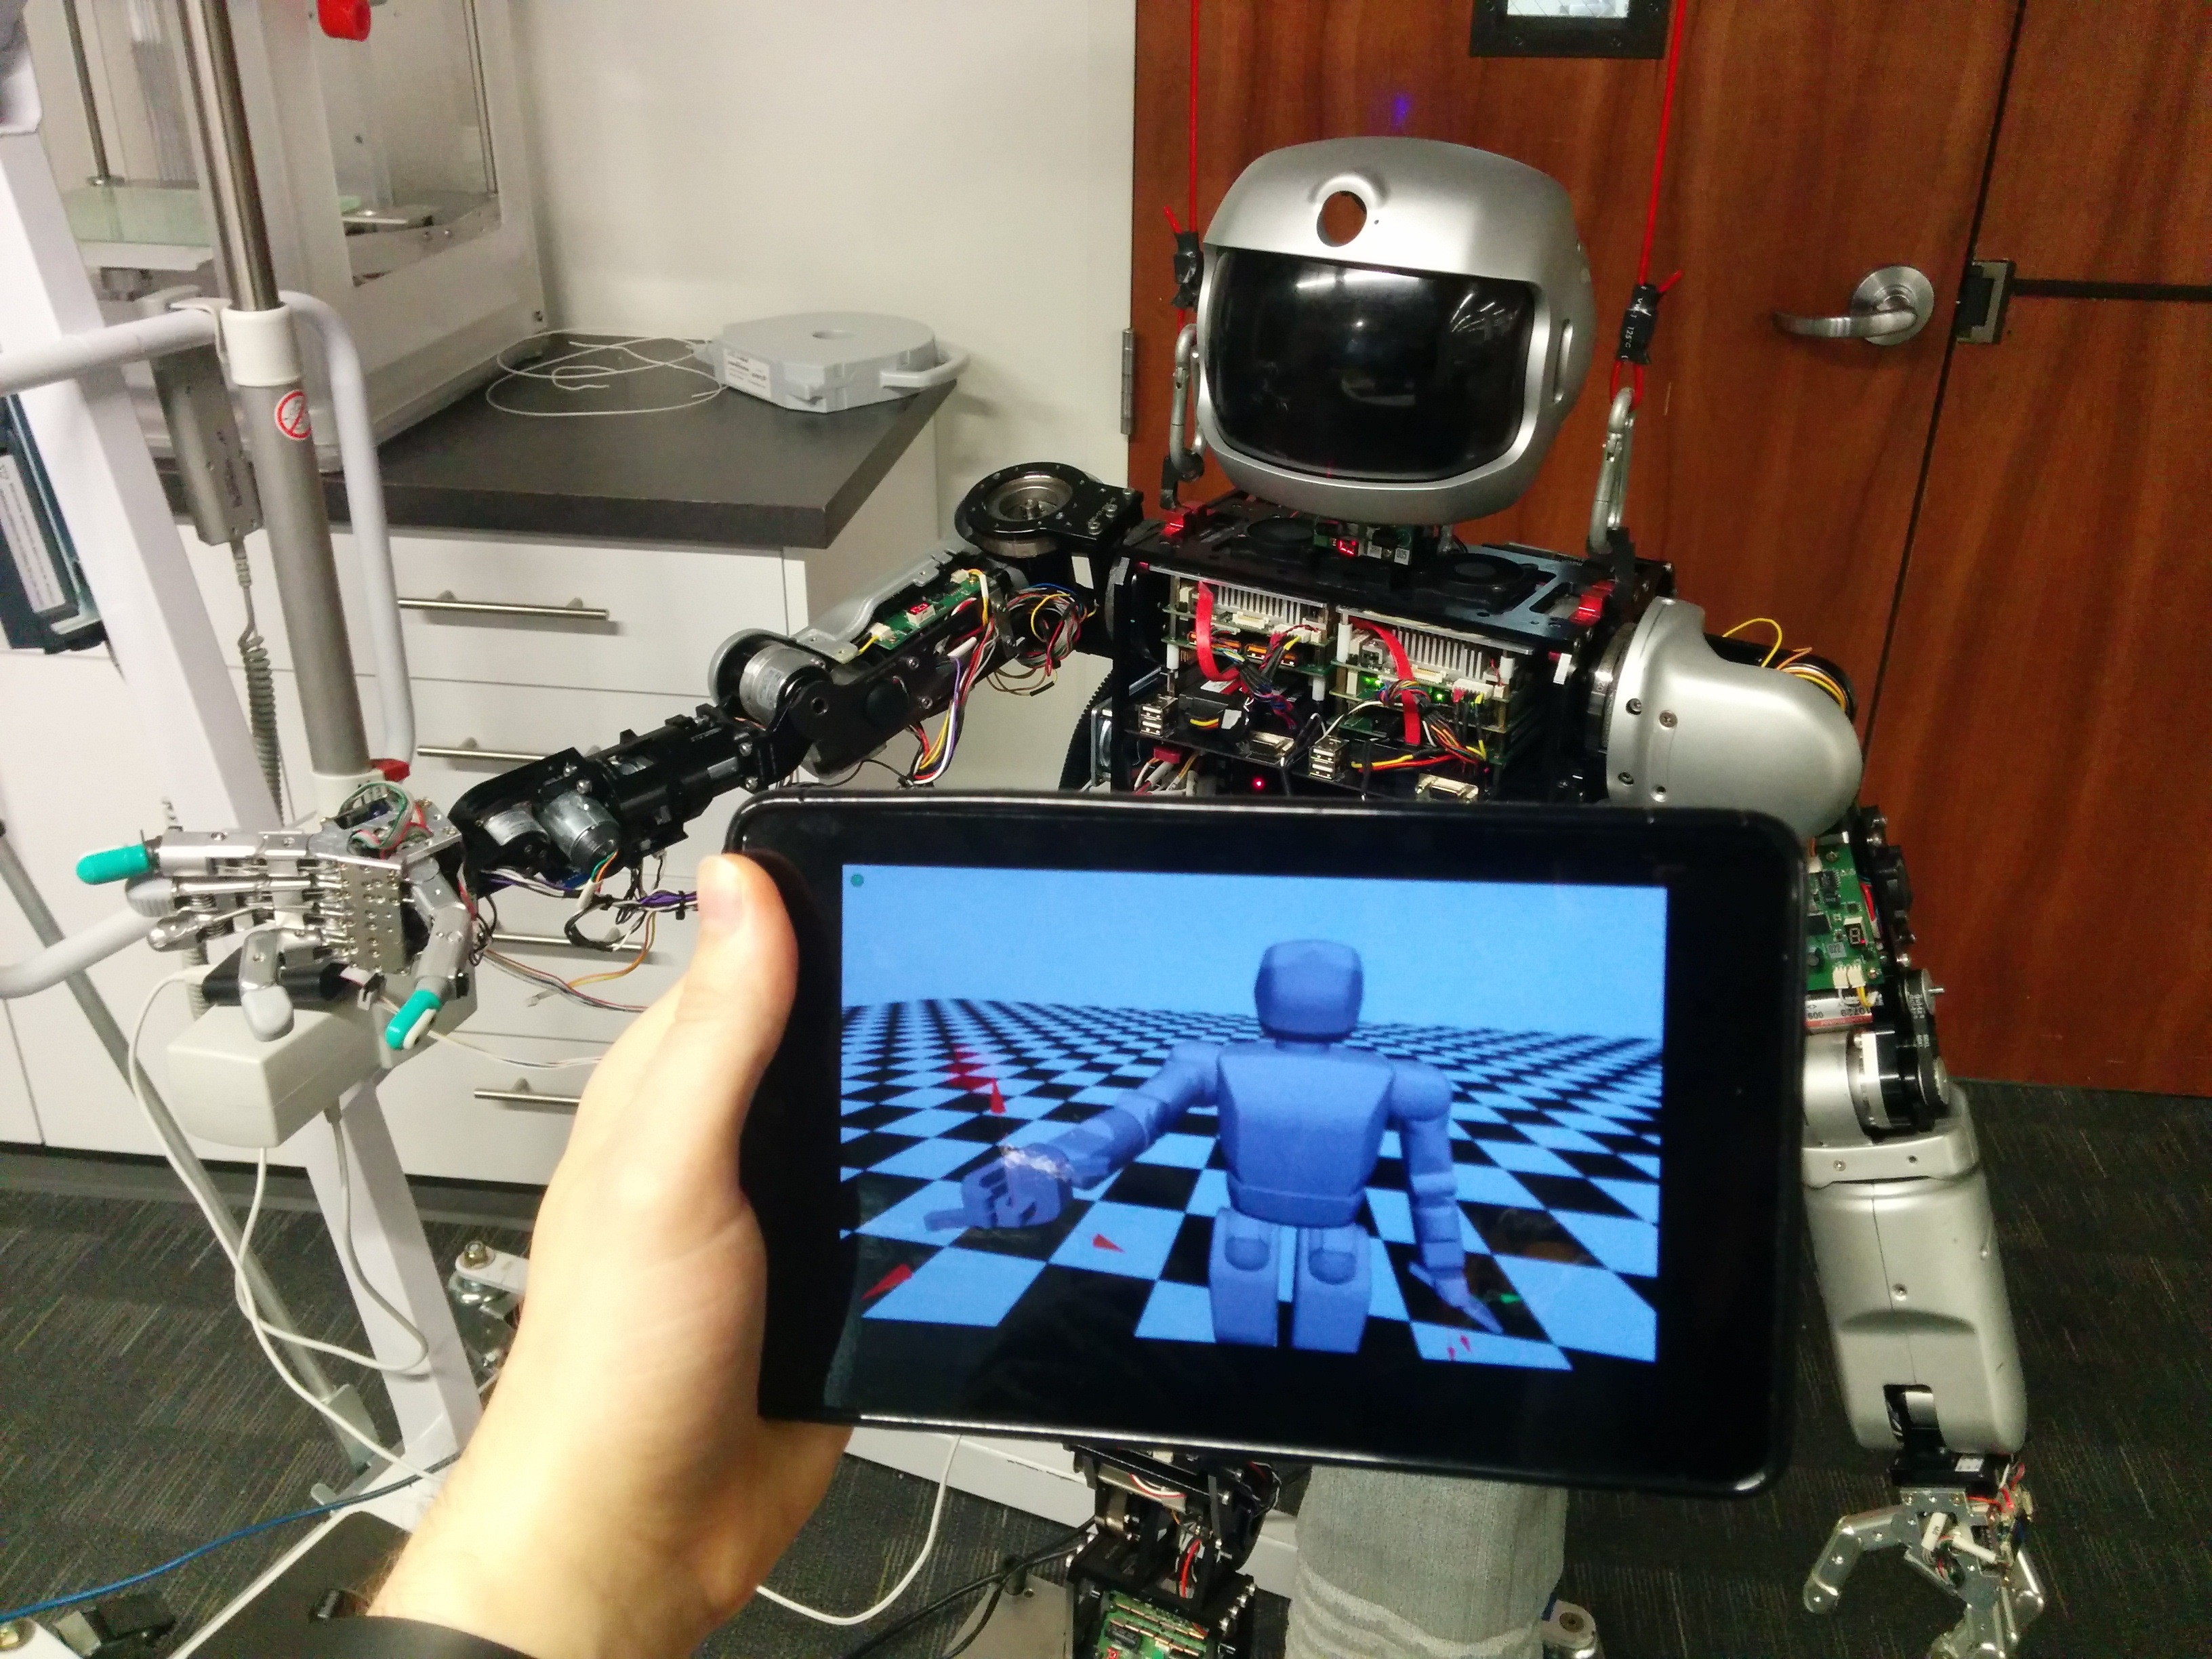
\includegraphics[width=3in]{figures/hubo.jpg}
  \caption{The WebGL interface for Hubo 2+ running on a Nexus 7 tablet in fullscreen mode.}
  \label{fig:Hubo2}
\end{figure}

% Cross-platform
% Zero install
%   for these platforms
% Mobile
%   tested on phone and tablet
% Runs on cloud services (public/private)
%   tested on both
% Increases situational awareness
% Tested on two platforms


% Connects people around the globe with your robot.
% Enables better sharing.
% Enables better collaboration.
% Lastly, we made it work on mobile.


%%%%%%%%%%%%%%%%%%%%%%%%%%%%%%%%%%%%%%%%%%%%%%%%%%%%%%%%%%%%%%%%%%%%%%%%%%%%%%%%
\section{RELATED WORK}
% We're focussing on monitoring remotely
% These are the ways its currently done
Robotics software for mobile systems is still in its infancy.
One example of early efforts to port traditional robot monitoring software to tablets is the recent work to write native Android version of \texttt{rviz}.
Due to the differences between the Android tablet environment and desktop Ubuntu, Rviz for Android had to be ``written almost entirely from scratch''. \cite{rviz_android}
This highlights the problem discussed in the Introduction with regard to writing native apps for mobile devices, which we avoid by writing a web app.
Because of this, our app is not limited to Android.
In writing the native version of \texttt{rviz} for Android,``limited support'' for both WebSockets and WebGL on Android and iOS devices is cited as a reason to write a native Android app.
However, \texttt{rviz} for Android was started in 2011, and things have changed.
% NOTE: Actually we don't use web sockets. :-/ Just Socket.IO
At the time of writing, WebSockets are supported by all major desktop and mobile browsers except Opera Mini and the stock Android browser.\footnote{\url{http://caniuse.com/websockets}}
Although WebGL is still not turned on in iOS, it is well supported by both Chrome and Firefox for Android.\footnote{\url{http://caniuse.com/webgl}}
WebGL is enabled for iAds on iOS, so hopefully it will be enabled for all websites in a future version of iOS. \cite{iAd}
We primarily used Chrome for our development.
Planning for the future then, we are proudly pushing forward with using WebSockets and WebGL for mobile web applications.

A successful example of using WebGL to create an interactive 3D web interface for robots is \texttt{ros3d.js} from the Robot Web Tools suite.
It loads models in Universal Robot Description Format (URDF) using the \textit{Three.js} library (which uses WebGL for rendering). \cite{alexander2012robot}
Another such project is \texttt{wviz}\footnote{\url{https://github.com/jihoonl/wviz}} which is a limited \texttt{rviz} implementation for the web browser using WebGL.
Yet another website, \url{mymodelrobot.appspot.com} by Igor Zubrycki, lets users edit URDF files and see the results in a WebGL visualization, enabling students to experiment with designing their own robot.
These tools use WebGL to visualize robots, but not on mobile devices.
Our solution appears to be the first to support robot meshes defined in STL format instead of Collada.
However, it currently lacks texture support found in \texttt{wviz} and \texttt{ros3d.js}.

% Borrowed rosbridge for inspiration.
The most popular robotics software collection of the moment is Robot Operating System (ROS). \cite{quigley2009ros}
However, mobile devices are low-powered and do not meet the system requirements to run ROS.
A workaround is needed then for mobile devices to interface with robots running ROS.
Rosbridge is a project designed to ease the interfacing of non-ROS systems with ROS systems. \cite{crick2011rosbridge}
The Rosbridge server converts ROS messages into plain text JSON formatted messages and uses Tornado, a Python web server, to send them to non-ROS over WebSockets.
Rosbridge has been used to make web interfaces that interact with remote ROS-enabled robots. \cite{pitzer2012pr2}
Notably, it has also been used to enable Android applications to communicate with ROS-enabled robots.
Tablet interfaces exploiting Rosbridge to talk to ROS-enabled robots include ``wheeled, air, surface, and underwater vehicles''.  \cite{speers2013diver}
However, Rosbridge has also been used to do the opposite: allow non-ROS robots to interface with ROS-enabled computers. \cite{dallaroslink} \cite{aznar2014ros}
Hubo is ROS compatible, so we might have used Rosbridge as our server backend.
However, we wanted to have more control over the bandwidth that the server used in order to get the fastest possible updates, and to supplement the WebSocket technolgoy used by Rosbridge with other frameworks like Firebase.
Therefore we borrowed inspiration from Rosbridge, but not the implementation.

%%%%%%%%%%%%%%%%%%%%%%%%%%%%%%%%%%%%%%%%%%%%%%%%%%%%%%%%%%%%%%%%%%%%%%%%%%%%%%%%
\section{METHODOLOGY}

\subsection{Overview of System}

Fig. \ref{fig:Overview} shows a general overview of the system.
Since it is a monitoring system, we can consider data starting at the robot and flowing to the client interface.
As shown in the diagram, both private and public cloud configurations were developed and tested.
The robot, sniffer, and client interfaces are described in more detail that follows.

\begin{figure}[thpb]
  \centering
  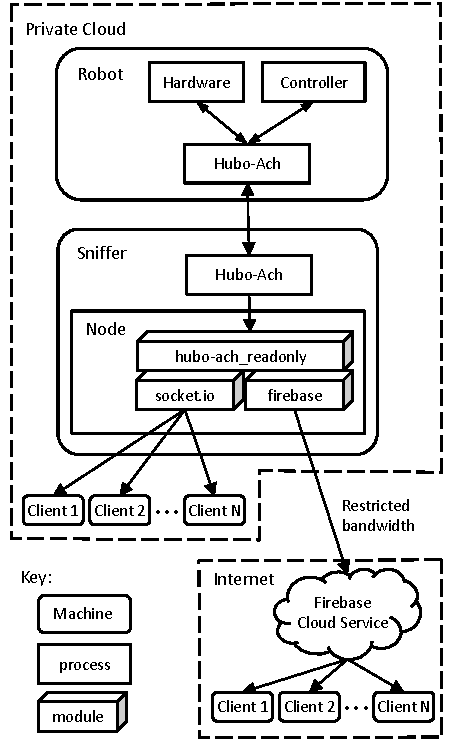
\includegraphics{figures/DetailedOverview.pdf}
  \caption{Detailed overview of system}
  \label{fig:Overview}
\end{figure}

\subsection{Robot}
% Transition to CAN-bus etc is too jarring.
% Put in a paragraph called "Robot" or something

Both Hubo robots are controlled by body computers located in the robot's torso, which communicate via a controller area network (CAN) bus with motor control boards that control the motors.
The body computer runs Ubuntu 12.04 Linux.
The control software for Hubo is developed using Hubo-Ach, a framework that handles communicating with the motors over the CAN-bus.\cite{lofaro2013unified}
Hubo-Ach communicates with other processes such as the controller and motion planner via the ACH IPC, which is based on memory mapped files.\cite{dantam2012robust}
Hubo-Ach has remote functionality allowing up to 1kHz communications between computers over Ethernet.
By using Hubo-Ach's remote abilities, we can offload the web server component of our system to another computer, freeing resources on the Hubo body computer.
This second computer is the ``Sniffer'' because it reads from the Hubo-Ach channel.
The sniffer computer acts as the server for our interface.

\subsection{Server Implementation}
%- Some won't be familiar with WebGL and WebSockets.  You should provide at least a brief description / definition.
The primary of the system design was to be highly portable and zero installation.
Because the client interface is web-based, the only part of the system that has to be installed is the server.
(The server is labeled ``Sniffer'' in Fig. \ref{fig:Overview} because it sniffs the robot state from the hubo-ach channel.)
Traditional HTTP servers such as Apache can be complicated to install and configure, particularly if the server-side logic requires installing additional environments such as PHP.
For our implementation, we used a platform called \textit{Node}\footnote{\url{http://nodejs.org/}} as the backend.

Node is a platform built on top of the V8 JavaScript engine used in Google Chrome.
It includes an HTTP server in its core modules, and many user-written modules are available.
All modules are installed by the built-in package manager that comes with Node, called \texttt{npm}.
This makes it very easy to specify the dependencies of a piece of software and install them, regardless of what OS you run Node on.

The authors support open source software development.
Thus all of the source code for our interface is available at: \url{https://bitbucket.org/wmhilton/drchubo.js}
The server software was tested on Ubuntu 12.04 LTS because that is what our lab uses to operate our Hubo robots.
However, the client side of course is cross-platform and supported by multiple browsers and operating systems.

The sniffer publishes robot states at a periodic interval.
After optimizing the performance as described in the next section, we were able to achieve updates at 30 frames per second (FPS).
An update rate of 30 FPS resulted in very smooth animations in the interface that were pleasing to the eye.
However, for practical purposes the framerate was reduced to 10 FPS because a human's reaction time is no better than 1/10th of a second, so faster frame rates (while aesthetically pleasing) were not of much practical value for monitoring the robot. \cite{kosinski2008literature}
This cut down on bandwidth.

How the sniffer publishes robot state data depends on whether you are running the server in ``public cloud'' or ``private cloud'' mode.
In private cloud mode, the sniffer publishes state data using a library called Socket.IO\footnote{http://socket.io}.
On the server side this is a Node module, and on the client side it is a JavaScript file you include in the webpage.
Socket.IO provides an abstract socket that can be used to pass asynchronous messages between the client and server without having to refresh the webpage.
On modern browsers this socket is implemented using HTML5 WebSocket technology, but because Socket.IO has multiple fallback technologies, it will work with browsers as old as Internet Explorer 5.5 or Firefox 3.
Using Socket.IO allows us to run the user interface on a local network without any external Internet connection.

In public cloud mode, we use a different mechanism for publishing state data.
If hundreds or thousands of users across the globe are using the system, we do not want the burden of serving such large traffic loads to fall on the sniffer computer.
In fact, the connection between the local robot network and the Internet will generally have a finite bandwidth, limited by a WiFi router or similar.
Instead of connecting to all those browsers the sniffer computer, we employ a third-party cloud service called Firebase.
Firebase provides a persistent tree-like structure ``database'' where any change made to the database by one client is (almost) instantly reflected in all the other clients (e.g. it synchronizes the data between clients).
It can be used for multi-directional communication between instances of web applications running on web browsers.
In the current web interface though, we are just using it for server-to-client communication.
The sniffer only maintains one connection, to Firebase's servers.
When the Firebase is updated, any running instances of the client interface are notified with the updated data.

The client interface consists of static HTML, CSS, and JavaScript files.
In private cloud mode, the sniffer can also act as the host for the web interface, using Node as an HTTP server.
The users simply type in the IP Address of the sniffer computer into their web browser.
In public cloud mode, the client interface files can be hosted by any hosting provider.
Because the web interface contains a hardcoded URL pointing to the Firebase where state data updates are, it doesn't matter what the address of the client interface is.
One can host the web interface on a lab website, or a provider such as Github Pages.

\subsection{Client Interface}
We chose to write the client in HTML5 + JavaScript in order to be cross-platform, zero-install, and future-proof.
The goal of our interfaces was to improve situational awareness of the robot operator, who may or may not be within a line of sight of the robot, and provide useful debugging information about the robot's motors.

There are two interfaces we developed.
The first, shown in Fig. \ref{fig:Qualitative}, is a graphical interface that shows the pose, orientation, and force-torque data of the robot as a 3D model that can be rotated, panned, and zoomed.
The second, shown in Fig. \ref{fig:Quantitative}, is a plain text interface, which shows the joint reference positions, encoder values, sensor data, and motor board error flags in a table.
These two representations complement each other: the 3D interface shows the big picture, and the plain text interface provides the fine details.

\begin{figure*}[ptb]
    \centering
    \begin{subfigure}[b]{2.5in}
        \centering
        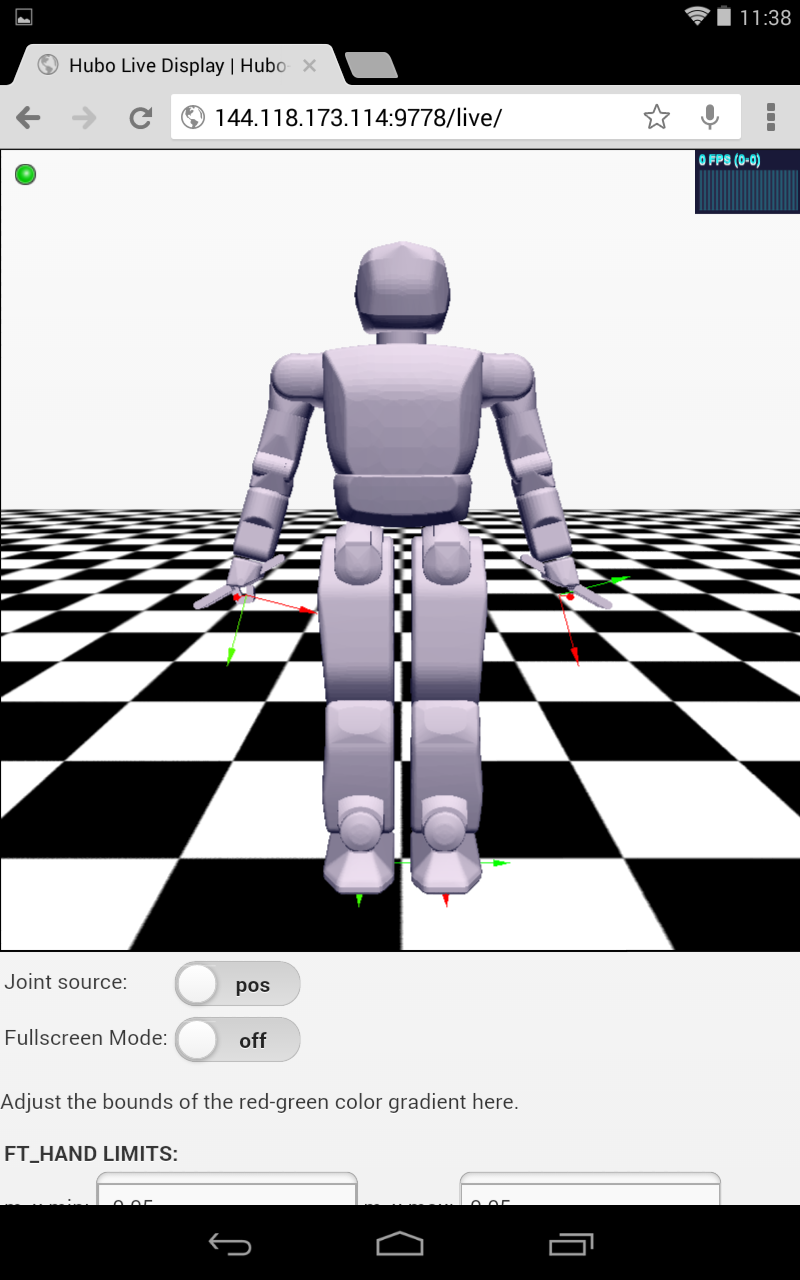
\includegraphics[width=2in]{figures/QualitativePortrait.png}
        \caption{The WebGL interface displays the robot's pose as well as force-torque data.}
        \label{fig:Qualitative}
    \end{subfigure}%
    \quad
    \begin{subfigure}[b]{2.5in}
        \centering
        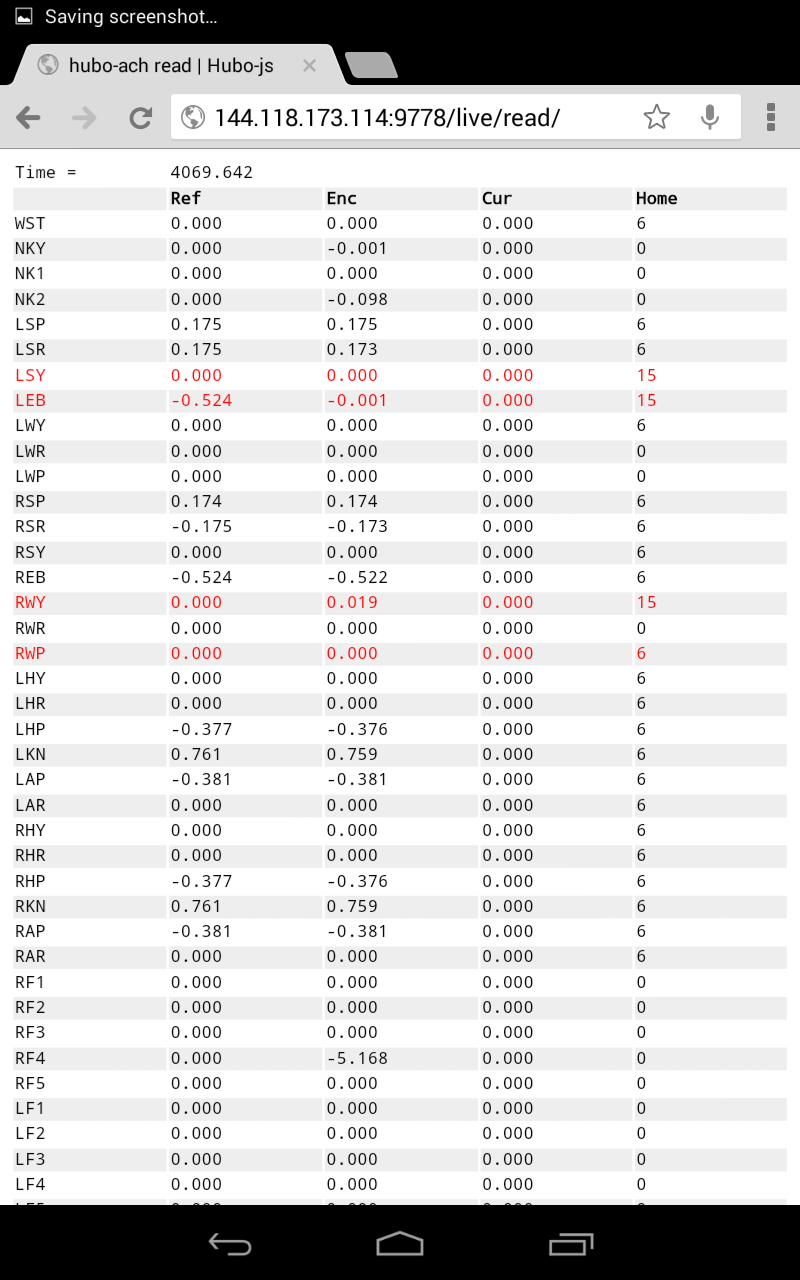
\includegraphics[width=2in]{figures/QuantitativePortrait.png}
        \caption{The plain text interface displays detailed data about each joint. }
        \label{fig:Quantitative}
    \end{subfigure}%
    \caption{Screenshots of the interfaces on a Nexus 7 tablet.}
    \label{fig:Screenshots}
\end{figure*}

The WebGL interface is useful for getting an overall sense of the robot's state.
Visualizations are much more efficient for humans than reading raw numbers.
We can more easily see problems, discrepancies, etc.
The plain text interface is useful for debugging and includes the status of individual motor boards.
When it becomes apparent that a joint is not moving or a force torque sensor is miscalibrated, examining the numbers in the raw plain text display provides insight.

The 3D models used by this visualization tool come from the OpenHubo project.\cite{lofaro2012humanoid}
They are the same URDF models used in the OpenHubo robot simulator that is based on OpenRAVE.
To import the model into the browser, we wrote a JavaScript fucntion to parse the URDF file for the model and load the individual body meshes using the \textit{Three.js} library.\footnote{\url{threejs.org}}
Both meshes in Collada or STL format are supported.
From the kinematic information in the URDF file, we automatically construct a hierarchical virtual robot object.
Within this virtual robot object is an array of joint objects.
Changing the value property of the joint object triggers a function that rotates the appropriate links and re-renders the robot.
To improve efficiency, in practice we disable auto re-rendering and only re-render the robot once all of its joints have been updated.
Because the kinematic models for the robot are not hard-coded by loaded dynamically, it was straightforward for us to develop the same app for both Hubo 2+ (Fig. \ref{fig:Hubo2}) and DRC-Hubo (Fig. \ref{fig:DRCHubo}).

\begin{figure}[thpb]
  \centering
  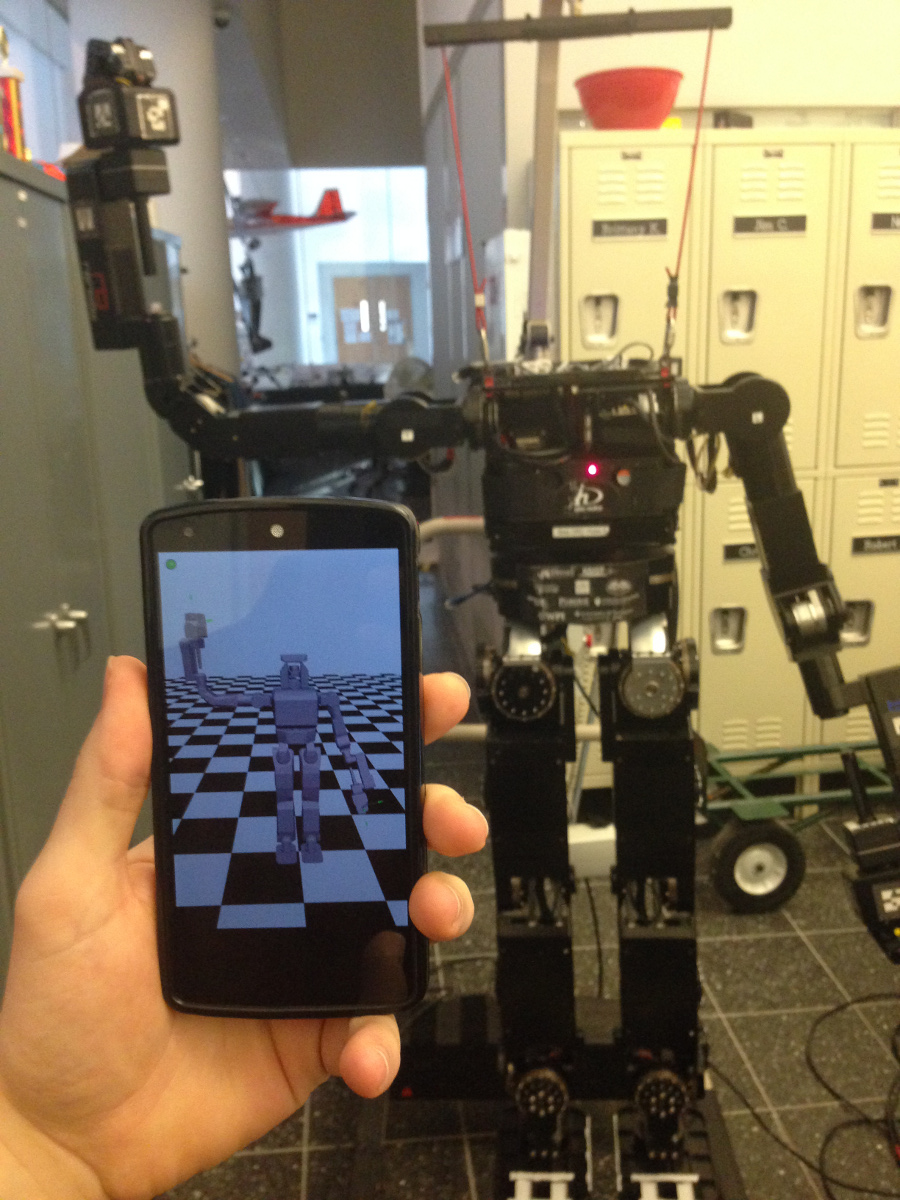
\includegraphics[height=3in]{figures/drchubo.jpg}
  \caption{Testing the fullscreen WebGL interface for DRC Hubo running on a Nexus 5 phone.}
  \label{fig:DRCHubo}
\end{figure}

%\begin{figure*}[ptb]
%    \centering
%    \begin{subfigure}[b]{3in}
%        \centering
%        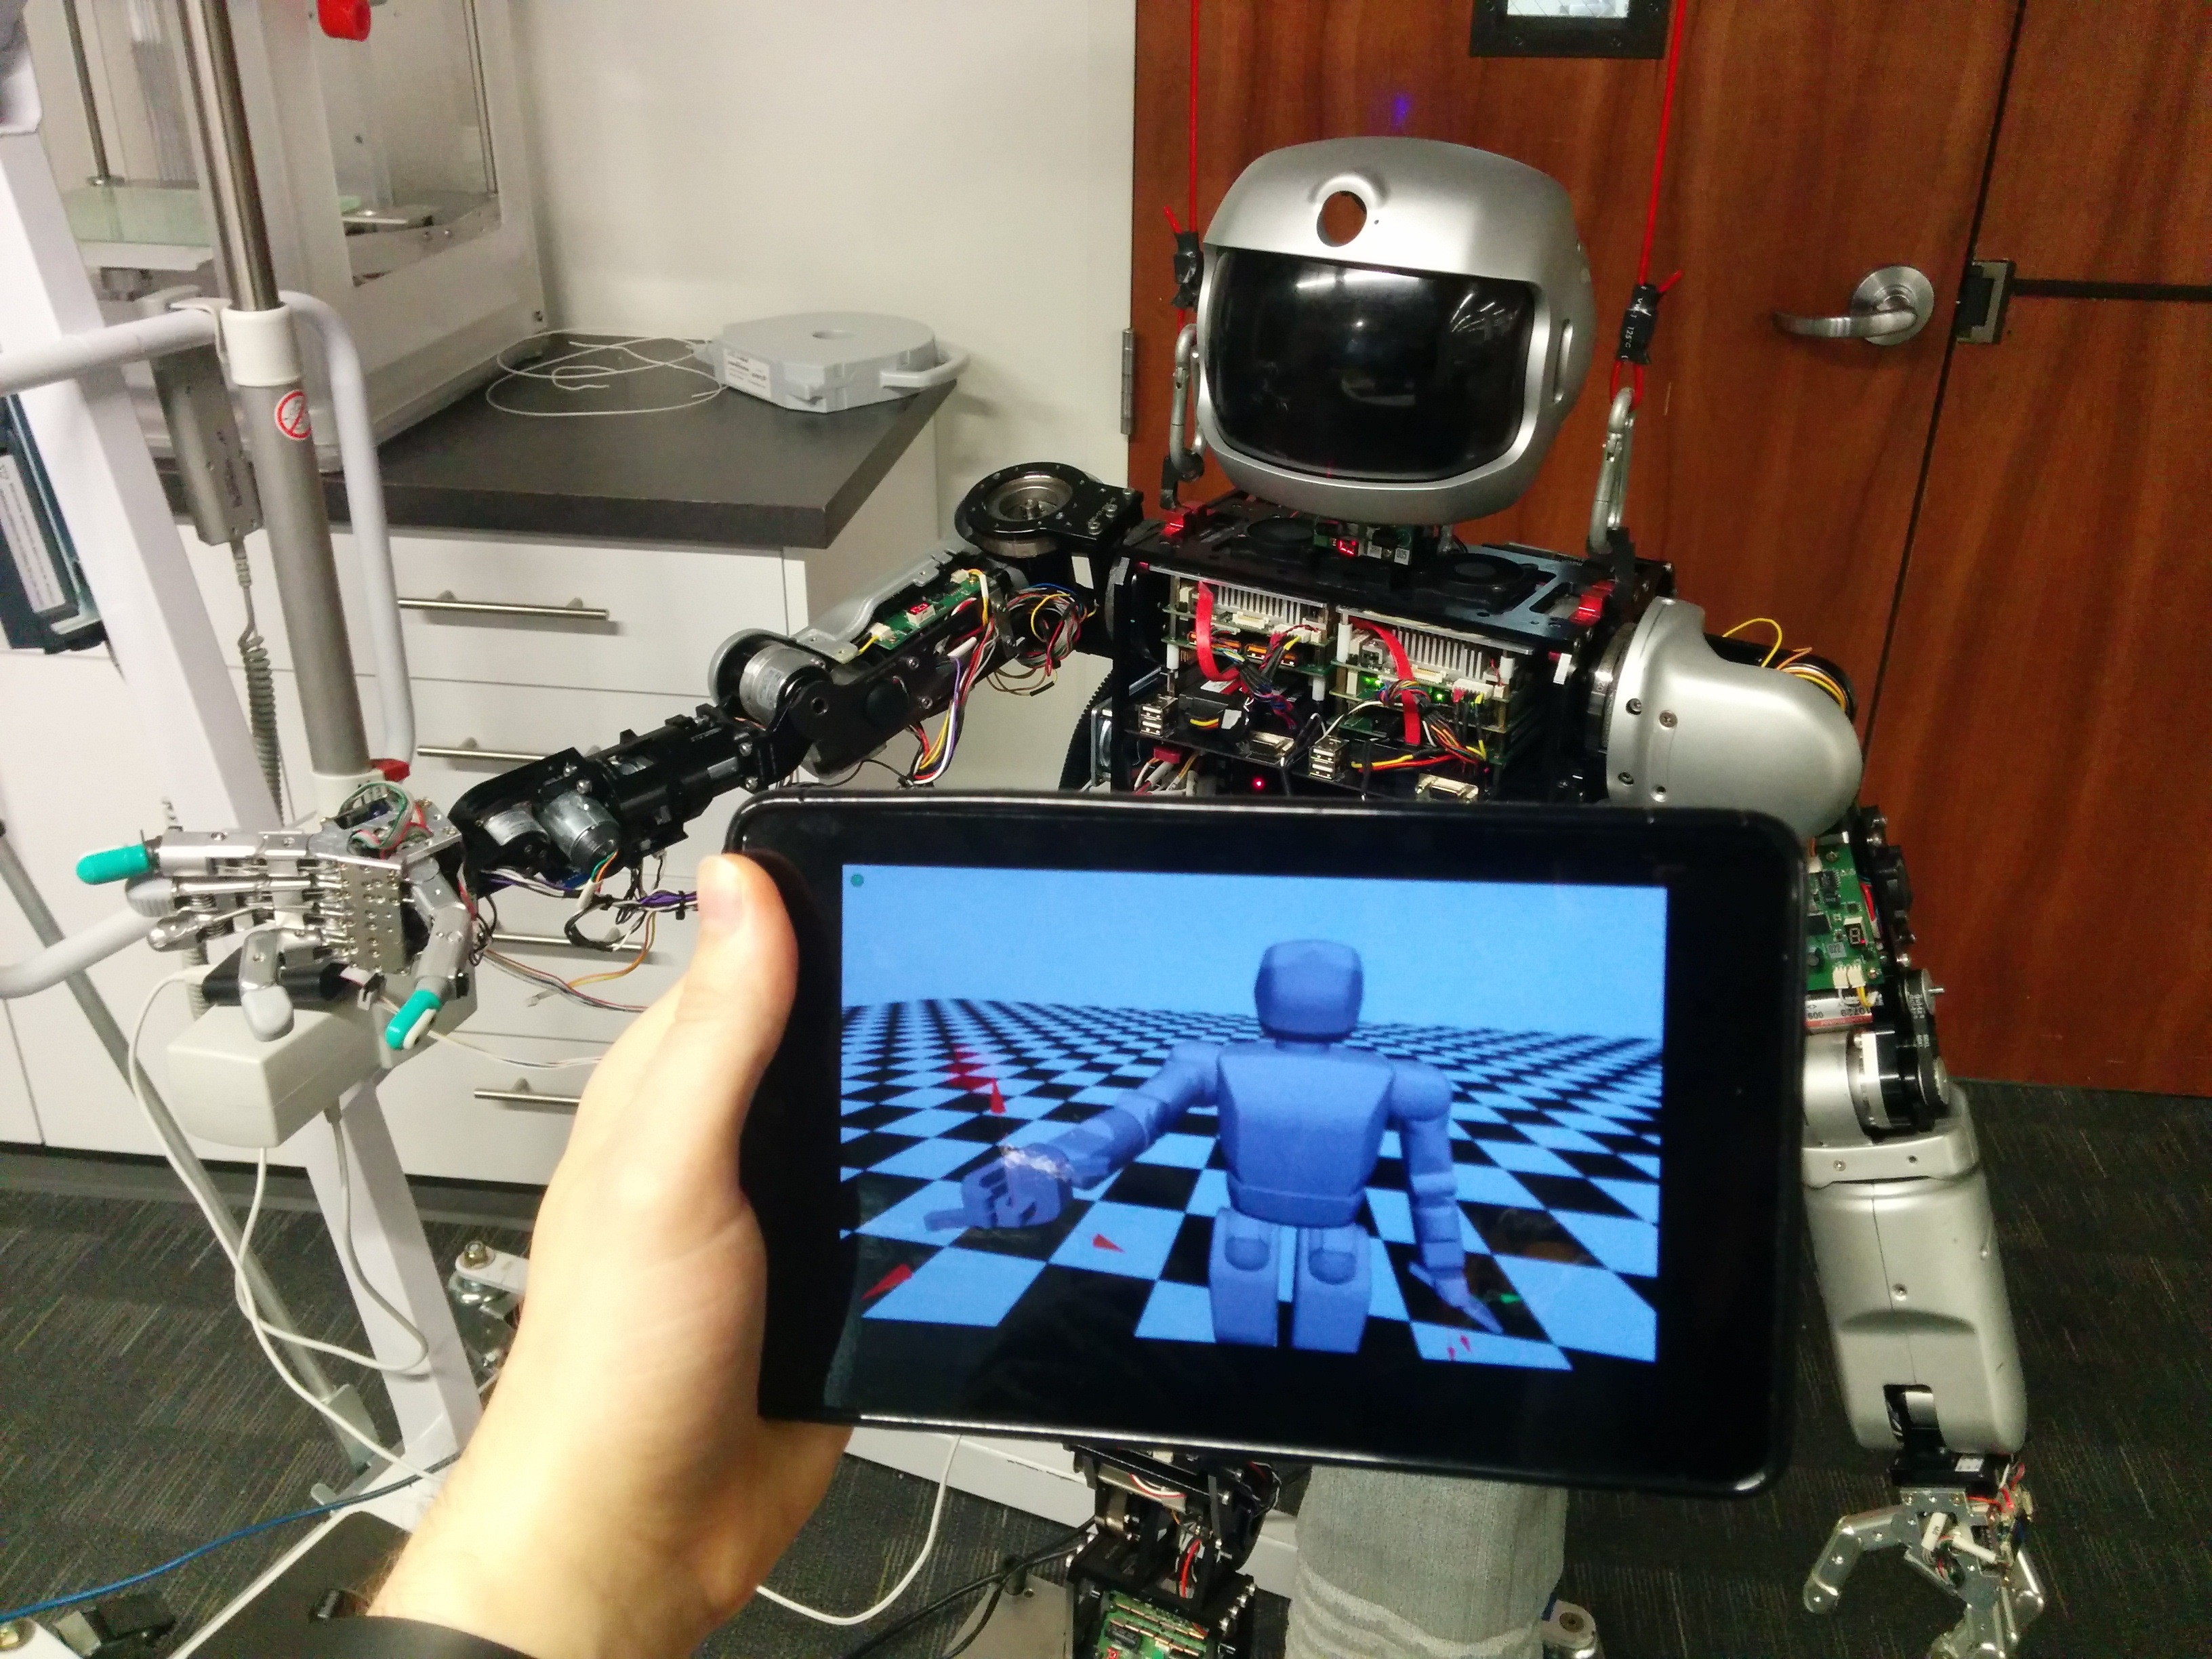
\includegraphics[width=3in]{figures/hubo.jpg}
%        \caption{Demo on a Nexus 7 tablet in front of Hubo 2+.}
%        \label{fig:Hubo}
%    \end{subfigure}%
%    \quad
%    \begin{subfigure}[b]{3in}
%        \centering
%        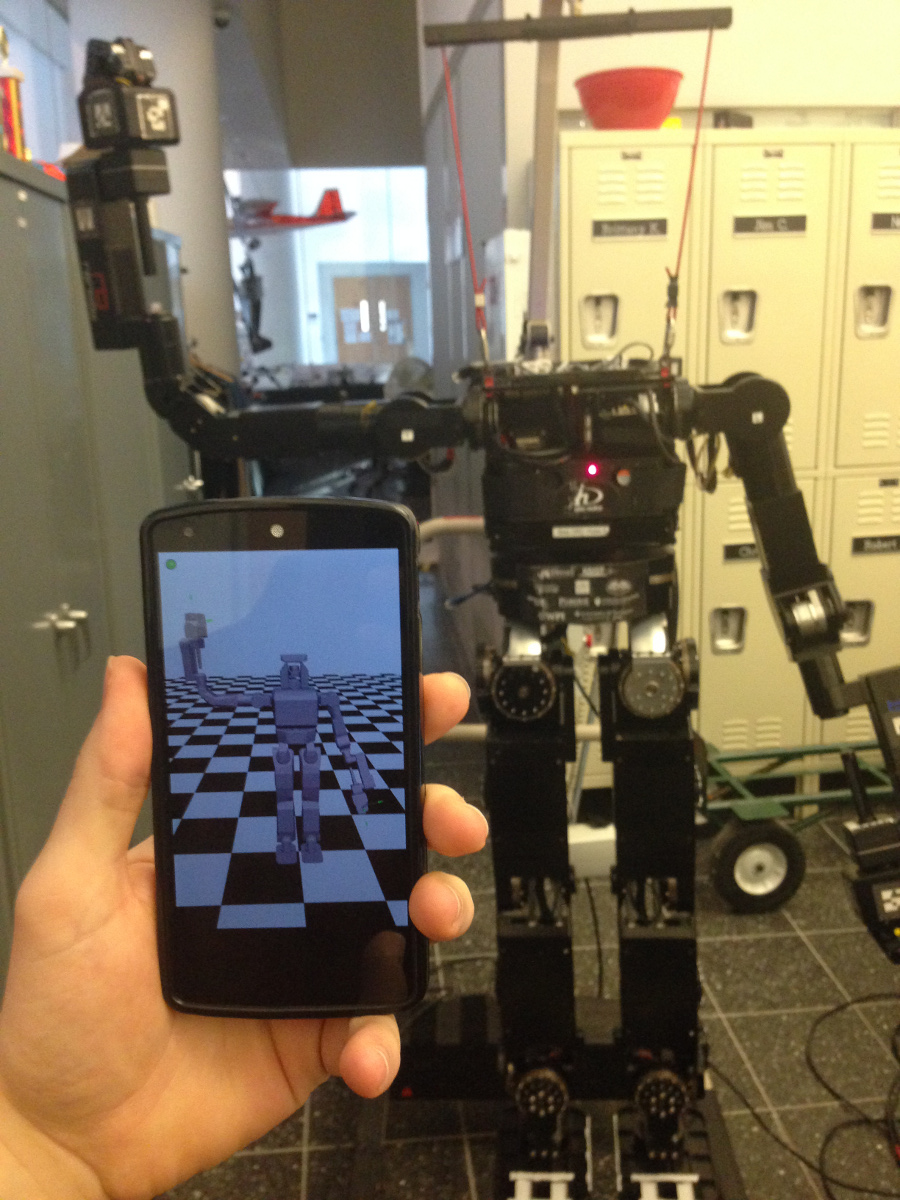
\includegraphics[height=3in]{figures/drchubo.jpg}
%        \caption{Demo on a Nexus 5 phone in front of DRC Hubo.}
%        \label{fig:DRCHubo}
%    \end{subfigure}%
%    \caption{Photos of the WebGL display in full screen mode in front of the robot(s).}
%    \todo[inline]{Are these good enough?}
%    \label{fig:Photos}
%\end{figure*}

The following sections describe the data visualizations in more detail.

\subsubsection{Joint Angles}
% Goals: is the robot over-torquing itself
% Is it in desired pose 
% This allows the user to easily see this and use their smarts
The interface visualized joint angles by setting joint angles on the WebGL robot model.
The interface lets users toggle between two sets of angles:
\begin{itemize}
\item The ``pos'' or position angles: the angles reported by the joint encoders.
\item The ``ref'' or reference angles: the commanded angles, i.e. the set point for the controllers. 
\end{itemize}
Toggling between the two views immediately reveals any large discrepancy between the desired joint angles and the actual angles.
This can reveal whether motors are being over-torqued.
Discrepancies tend to happen when there is a motor malfunction causing a motor to stop moving, or if an obstacle is preventing a limb from reaching its target pose.

Another situation where discrepancies occur is when certain joints are set to be in a compliant mode.
During walking, for instance, DRC Hubo will enable compliance in the shoulder joints allowing the arms to swing side to side.
This could be observed in the ``pos'' mode, but not in the ``ref'' mode since the arms were not being commanded to swing.

An alternative to having a toggle switch is to show both sets of angles at once using two robot models, where one or both models are partially transparent.
This is the approach used in OpenHubo.
This could have been done in the web app as well, at the cost of doubling the amount of geometry that needs to be rendered.

In the plain text interface, more information about joints are available.
The joint's three letter acronym is on the far left.
To the right, are quantities that are harder to show on the 3D model, like the amount of current being used and the exact value of the encoder and reference angles.
Most useful to us, we shows the "Homing flag" reported by the motor control board, indicating whether the joint is homed correctly.
Joints whose motor control boards report an error (such as over-torqued or over-saturated) are highlighted in red.

\subsubsection{Force Torque Sensors}
Both Hubo 2+ and DRC Hubo have force-torque sensors in the wrists and ankles that measure the normal force and the two moments perpendicular to the normal force.
These measurements were visualized as vectors emanating from the hands and feet of the robot, seen in Fig. \ref{fig:FT}).

\begin{figure}[thpb]
  \centering
  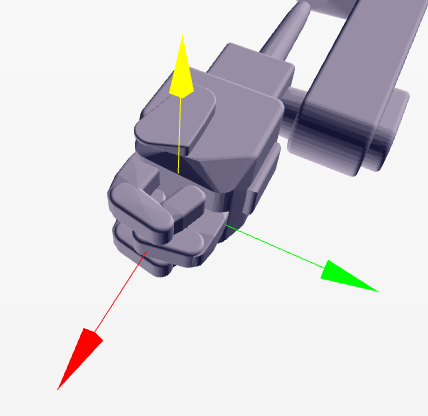
\includegraphics[width=1.5in]{figures/FT.png}
  \caption{Visualization of the force-torque data}
  \label{fig:FT}
\end{figure}

The primary goal of the force-torque visuals was to alert the monitoring user if too much force was being exerted on the ankles and wrists.
Therefore the force-torque vectors' colors are mapped to green, yellow, or red. 
Green means the force is within a safe range, red means too much, and yellow means in between.
The exact values to use as thresholds between green, yellow, and red can be set by the user in the web interface.

\subsubsection{Inertial Measurement Unit}
Both Hubo 2+ and DRC Hubo have one inertial motion unit (IMU) in the torso and one in each leg.
The torso IMU was visualized in the WebGL interface; however, all 3 IMUs were displayed in the plain text interface.
The primary use of the torso IMU was to indicate the orientation of the robot against the ground.
Of all the data to be monitored, this is one of the most important, particularly for tasks like ladder climbing and walking.
A poor orientation could indicate the robot was not well placed or did not have a good grip on the ladder.
At any time, orientation gives a good indication of whether the robot is tipping or has fallen.
% Through experience, it is beneficial to increase the users situational awareness if there is no line-of-sight.
Because the monitoring user could rotate the 3D graphical model of the robot in all three axis, the orientation of the robot on the screen was not sufficient indication of the robot's orientation in real life.
To properly visualize the orientation of the robot, a reference plane was inserted in the visualization at the robot's foot level.
% Make "better situational awareness" a key focus issue of the paper. One of the goals mentioned originally.

\subsection{Optimization}
While the primary components of the system (Three.js, Node, and Firebase / Socket.IO) are all relatively easy to use, optimizations on the client and server were needed to achieve the high throughput and smooth rendering performance of our system.
The initial prototype of the system relied naively on the Firebase API.
On the server side, it would upload a JSON structure of the robot state every update.
On the client side, event handlers were triggered for every updated joint.
This was a simple and intuitive scheme.
However, the initial prototype of the system did not perform well, and experienced severe lag (up to several seconds) and could cause the browser to hang.
This was largely due to the fact that dozens of asynchronous events were being triggered for what was really just one state update.
In later versions of the system, instead of using one message per joint / sensor, all the data was serialized into JSON format and sent as a single string.
Thus on the client end, only a single function was run once per update.
The event handler would deserialize the data, update the joint rotations of the 3D model, and then render the model.

Because Firebases have a fixed amount of bandwidth per month (5GB for the free developer plan), to further reduce bandwidth, the server only sends out messages if the state of the robot changes.
In fact, we round all the state values to 3 decimal places during the serialization to eliminate state changes caused by encoder noise.
The server only transmits the serialized data if the message string is different from the previous message string.
When the private cloud option was developed using Socket.IO, this helped free up local bandwidth for other devices.

%%%%%%%%%%%%%%%%%%%%%%%%%%%%%%%%%%%%%%%%%%%%%%%%%%%%%%%%%%%%%%%%%%%%%%%%%%%%%%%%
\section{RESULTS}
%- Additional qualitative feedback about performance would be helpful here.  I'm guessing that it still performs (feels) better on some platforms vs. others.
The interface was tested on a variety of platforms to verify its cross-platform compatibility.
These tests were done using the private cloud interface (i.e. the socket.io backend, not the Firebase backend).
For mobile testing, we used a Nexus 5 smartphone and the Nexus 7 tablet by Google.
For desktop testing, we used the author's laptop, which happens to be a Toshiba Portege z835 ultrabook.
Testing for OSX and iOS were done on Apple hardware for obvious reasons.
The results of desktop testing are shown in Table \ref{tab:DesktopTesting}.
The results of mobile testing are shown in Table \ref{tab:MobileTesting}.
In general, the desktop browsers that supported WebGL all felt equally good.
However, on the mobile testing, it felt like Chrome did smoother rotate/pan/zoom than Firefox.

\begin{table}[h]
\begin{center}
\begin{threeparttable}[b]
\caption{Desktop Testing}
\label{tab:DesktopTesting}
\begin{tabular}{|c|c|c|c|c|c|}
\hline         & \multicolumn{4}{|c|}{Windows 7 (Toshiba Portege z835)} & \multicolumn{1}{|c|}{OSX} \\ 
\hline          & IE 11            & Chrome 32 & Firefox 26 & Opera 19 & Safari 7 \\ 
\hline Hubo 2+  & \xmark \tnote{1} & \cmark    & \cmark     & \cmark   & \cmark  \tnote{2} \tnote{,3} \\ 
\hline DRC Hubo & \cmark \tnote{2} & \cmark    & \cmark     & \cmark   & \cmark  \tnote{2} \tnote{,3} \\ 
\hline 
\end{tabular} 
\begin{tablenotes}
\item [1] Hubo 2+ doesn't work in IE because the COLLADA file loader is broken in IE. DRC Hubo uses STL files so it works.
\item [2] Fullscreen mode doesn't work.
\item [3] WebGL has to be enabled in the ``Develop'' menu.
\end{tablenotes}
\end{threeparttable}
\end{center}
\end{table}
\begin{table}[h]
\begin{center}
\begin{threeparttable}[b]
\caption{Mobile Testing}
\label{tab:MobileTesting}
\begin{tabular}{|c|c|c|c|c|c|c|}
\hline         & \multicolumn{4}{|c|}{Android 4.4 (Nexus 5)} & \multicolumn{2}{|c|}{iOS 7 (iPad 2)} \\ 
\hline         & Chrome & Firefox          & Dolphin          & Opera  & Chrome           & Safari \\ 
\hline Hubo 2+ & \cmark & \cmark \tnote{1} & \xmark \tnote{2} & \cmark & \xmark \tnote{2} & \xmark \tnote{2} \\ 
\hline DRC Hubo& \cmark & \cmark \tnote{1} & \xmark \tnote{2} & \cmark & \xmark \tnote{2} & \xmark \tnote{2} \\ 
\hline 
\end{tabular} 
\begin{tablenotes}
\item [1] There is noticeable lag in the touch interface however.
\item [2] Lack of WebGL results in unresponsiveness.
\end{tablenotes}
\end{threeparttable}
\end{center}
\end{table}

%%%%%%%%%%%%%%%%%%%%%%%%%%%%%%%%%%%%%%%%%%%%%%%%%%%%%%%%%%%%%%%%%%%%%%%%%%%%%%%%
\section{CONCLUSIONS & FUTURE WORK}
% Cross-platform
% Increases situational awareness
We have developed a cross-platform system for monitoring high degree of freedom robots to improve the situational awareness of the robot operators.
% Zero install
%   for these platforms
By creating a web interface, we have eliminated the need for users to install any special software.
% Mobile
%   tested on phone and tablet
The system works well on both desktop and mobile devices, and has been tested successfully on laptops, the Nexus 5 smartphone, and the Nexus 7 tablet.
% Runs on cloud services (public/private)
%   tested on both
The system has been tested in both private and public cloud configuration.
% Tested on two platforms
Finally, the interface has been tested on two hardware platforms, the Hubo 2+ and DRC Hubo.

One of the advantages of using the \textit{Three.js} library for rendering is that there is a software rendering fallback if WebGL is not supported in the browser.
In the future, we could adapt to the users' browser by detecting if WebGL is unavailable, and downloading a special ``low polygon count'' version of the robot that will render efficiently on browsers using software rendering.
This will increase the number of devices supported.

The system described in this paper only addresses monitoring from the robot.
We have been working on another web interface that interfaces to a simulation environment, in which users can control the robot.
We are currently working on how to safely close the loop, so that users can control the robot from the interface.
Future work will involve how to deal with multiple users all connected to the robot and trying to control it at the same time.
Negotiating which client has control of the robot, or deciding how multiple users can do simultaneous control, are ongoing research.

Lastly, we hope to make the system useful to a wider audience by integrating it with more types of robots.
The 3D interface already works with ROS's URDF format so many types of robots could be loaded into the interface, such as DARwIn-OP, Nao, PR2, and Baxter.
Since the underlying Websocket technology is similar to that used by the Rosbridge suite, we are looking at adapting the interface to work with the Rosbridge suite.


%%%%%%%%%%%%%%%%%%%%%%%%%%%%%%%%%%%%%%%%%%%%%%%%%%%%%%%%%%%%%%%%%%%%%%%%%%%%%%%%
\bibliographystyle{ieee/IEEEtran}
\bibliography{ieee/IEEEabrv,references}
\end{document}
